% Copyright (C) Data Structures and Algorithms Team.
\chapter{Heap}
A heap can be thought of as a simple tree data structure, however a heap usually employs one of two strategies:

\begin{enumerate}
\item min heap; or
\item max heap
\end{enumerate}

Each strategy determines the properties of the tree and it's values, e.g. if you were to choose the strategy min heap then each parent node would have a value that is $\leq$ than it's children, thus the node at the root of the tree will have the smallest value in the tree, the opposite is true if you were to use max heap. Generally as a rule you should always assume that a heap employs the min heap strategy unless otherwise stated.

Unlike other tree data structures like the one defined in \S\ref{bst} a heap is generally implemented as an array rather than a series of nodes who each have references to other nodes, both however contain nodes that have at most two children. Figure \ref{fig:tree_array_representation} shows how the tree (not a heap data structure) ($12~7$($3~2$)~$6$($9$~~)) would be represented as an array.

Using just an array is often not sufficient as we have to be upfront about the size of the array to use for the heap, often the run time behaviour of a program can be unpredictable when it comes to the size of it's internal data structures thus we need to choose a more dynamic data structure that contains the following properties:

\begin{enumerate}
\item we can specify an initial size of the array for scenarios when we know the upper storage limit required; and
\item the data structure encapsulates resizing algorithms to grow the array as required at run time
\end{enumerate}

\begin{figure}
\begin{center}
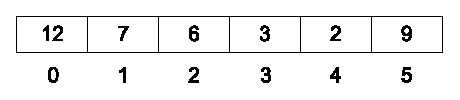
\includegraphics{heap_tree_array_representation}
\end{center}
\caption{Array representation of a simple tree data structure} \label{fig:tree_array_representation}
\end{figure}

The described data structure tends to have a named similar to:

\begin{enumerate}
\item Vector
\item ArrayList
\item List
\end{enumerate}

Because we are using an array we need some way to calculate the index of a parent node, and the children of a node, the required expressions for this are defined as follows:

\begin{enumerate}
\item ($index - 1$)/$2$ (parent index)
\item $2 * index + 1$ (left child)
\item $2 * index + 2$ (right child)
\end{enumerate}

In Figure \ref{fig:heap_tree_array_representation_indexes} a) represents the calculation of the right child of $12$ ($2 * 0 + 2$); and b) calculates the index of the parent of $3$ (($3 - 1$)/$2$).

\begin{figure}
\begin{center}
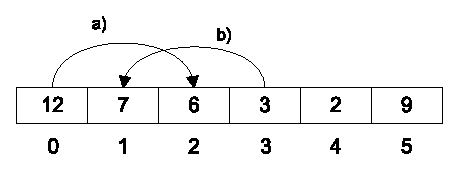
\includegraphics{heap_tree_array_representation_indexes}
\caption{Calculating node properties} \label{fig:heap_tree_array_representation_indexes}
\end{center}
\end{figure}

\section{Insertion}
Adding an item to a heap has an $O(log~n)$ run time complexity, this is due to the fact that after every insertion we must verify that the heap ordering strategy used is preserved, if not we must swap the values appropriately as we work up through the sub tree's starting with the sub tree the last value was added to.


Designing an algorithm for heap insertion is simple, however we must ensure that heap order is preserved after each insertion - generally this is a post insertion operation. Inserting a value into the next free slot in an array is simple, we just need to keep track of, and increment a counter after each insertion that tells us the next free index in the array. Inserting our value into the heap is the first part of the algorithm, the second is validating heap order which in the case of min heap ordering requires us to swap the values of a parent and it's child if the value of the child is $<$ the value of it's parent, we must do this for each sub tree the value we just inserted is a constituent of.

Figure \ref{fig:heap_insertion_minify_steps} shows the steps of inserting the values $3$, $9$, $12$, $7$, and $1$ into a min heap.

\begin{figure}
\begin{center}
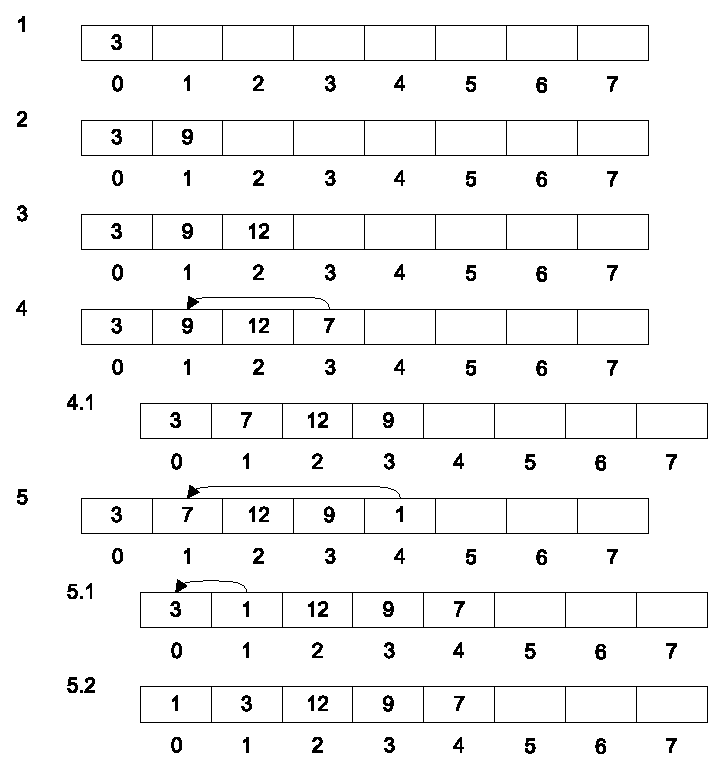
\includegraphics{heap_insertion_minify_steps}
\end{center}
\caption{Inserting values into a min heap} \label{fig:heap_insertion_minify_steps}
\end{figure}

\newpage
\begin{tabbing}
1)  \textbf{alg}\= \textbf{orithm} Add($value$) \\
2)  \> \textbf{Pre:}~~$value$ is the value to add to the heap \\
3)  \> ~~~~~~~~Count is the number of items in the heap \\
4)  \> \textbf{Post:}~the value has been added to the heap \\
5)  \> $heap$[Count] $\leftarrow value$ \\
6)  \> Count $\leftarrow$ Count $+ 1$ \\
7)  \> MinHeapify() \\
8)  \textbf{end} Add \\
\end{tabbing}

\begin{tabbing}
1)  \textbf{alg}\= \textbf{orithm} MinHeapify() \\
2)  \> \textbf{Pre:}~~Count is the number of items in the heap \\
3)  \> ~~~~~~~~$heap$ is the array used to store the heap items \\
4)  \> \textbf{Post:}~the heap has preserved min heap ordering \\
5)  \> $i \leftarrow$ Count $- 1$ \\
6)  \> \textbf{whi}\= \textbf{le} $i > 0$ \textbf{and} $heap$[$i$] $< heap$[($i - 1$)/$2$] \\
7)  \> \> Swap($heap$[$i$], $heap$[($i - 1$)/$2$] \\
8)  \> \> $i \leftarrow$ ($i - 1$)/$2$ \\
9)  \> \textbf{end while} \\
10) \textbf{end} MinHeapify \\
\end{tabbing}

The design of the \textit{MaxHeapify} algorithm is very similar to that of the \textit{MinHeapify} algorithm, the only difference is that the $<$ operator in the second condition of entering the while loop is changed to $>$. 

\section{Deletion}
Just like when adding an item to the heap, when deleting an item from the heap we must ensure that heap ordering is preserved. The algorithm for deletion has three steps:

\begin{enumerate}
\item find the index of the value to delete
\item put the last value in the heap at the index location of the item to delete 
\item verify heap ordering for each sub tree of that the value was removed from
\end{enumerate}

\newpage
\begin{tabbing}
1)  \textbf{alg}\= \textbf{orithm} Remove($value$) \\
2)  \> \textbf{Pre:}~~$value$ is the value to remove from the heap \\
3)  \> ~~~~~~~~$left$, and $right$ are updated alias' for $2*index+1$, and $2*index+2 $ respectively \\
4)  \> ~~~~~~~~Count is the number of items in the heap \\
5)  \> ~~~~~~~~$heap$ is the array used to store the heap items \\
6)  \> \textbf{Post:}~$value$ is located in the heap and removed, true; otherwise false \\
7)  \> // case 1 \\
8)  \> $index \leftarrow$ FindIndex($heap$, $value$) \\
9)  \> \textbf{if}~\= $index < 0$ \\
10) \> \> \textbf{return false} \\
11) \> \textbf{end if} \\
12) \> Count $\leftarrow$ Count $ - 1$ \\
13) \> // case 2 \\
14) \> $heap$[$index$] $\leftarrow heap$[Count] \\
15) \> // case 3 \\
16) \> \textbf{while} $2 * index + 1 <$ Count \textbf{and} $heap$[$index$] $> heap$[$left$] \textbf{or} $heap$[$index$] $> heap$[$right$] \\
17) \> \> // promote smallest key from sub tree \\
18) \> \> \textbf{if}~\= $heap$[$left$] $< heap$[$right$] \\
19) \> \> \> Swap($heap$, $left$, $index$) \\
20) \> \> \> $index \leftarrow left$ \\
21) \> \> \textbf{else} \\
22) \> \> \> Swap($heap$, $right$, $index$) \\
23) \> \> \> $index \leftarrow right$ \\
24) \> \> \textbf{end if} \\
25) \> \textbf{end while} \\
26) \> \textbf{return true} \\
27) \textbf{end} Remove \\
\end{tabbing} 

\section{Searching} \label{heap_searching}
Searching a heap is merely a case of traversing the items in the heap array sequentially, thus this operation has a run time complexity of $O(n)$. The search can be thought of as one that uses a breadth first traversal as defined in \S\ref{breadth_first} to visit the nodes within the heap to check for the presence of a specified item.

\newpage
\begin{tabbing}
1)  \textbf{alg}\= \textbf{orithm} Contains($value$) \\
2)  \> \textbf{Pre:}~~$value$ is the value to search the heap for \\
3)  \> ~~~~~~~~Count is the number of items in the heap \\
4)  \> ~~~~~~~~$heap$ is the array used to store the heap items \\
5)  \> \textbf{Post:}~$value$ is located in the heap, in which case true; otherwise false \\
6)  \> $i \leftarrow 0$ \\
7)  \> \textbf{whi}\= \textbf{le} $i <$ Count \textbf{and} $heap$[$i$] $!= value$ \\
8)  \> \> $i \leftarrow i + 1$ \\
9)  \> \textbf{end while} \\
10) \> \textbf{if} $i <$ Count \\
11) \> \> \textbf{return true} \\
12) \> \textbf{else} \\
13) \> \> \textbf{return false} \\
14) \> \textbf{end if} \\
15) \textbf{end} Contains \\
\end{tabbing}

\section{Traversal}
As mentioned in \S\ref{heap_searching} traversal of a heap is usually done like that of any other array data structure which our heap implementation is based upon, as a result you traverse the array starting at the initial array index (usually $0$ in most languages) and then visit each value within the array until you have reached the greatest bound of the array. You will note that in the search algorithm that we use \textit{Count} as this upper bound, not the actual physical bound of the allocated array. \textit{Count} is used to partition the conceptual heap from the actual array implementation of the heap, we only care about the items in the heap not the whole array which may contain various other bits of data as a result of heap mutation.
